%\chapter*{Неделя 3}
\protect\thispagestyle{fancy}
\section{}
Изобразить граф алгоритма БПФ с прореживанием \textbf{по частоте} для $N=16$. 
Объяснить, в чем заключается базовая операция данного алгоритма.

\begin{figure}[!h]
	\centering
	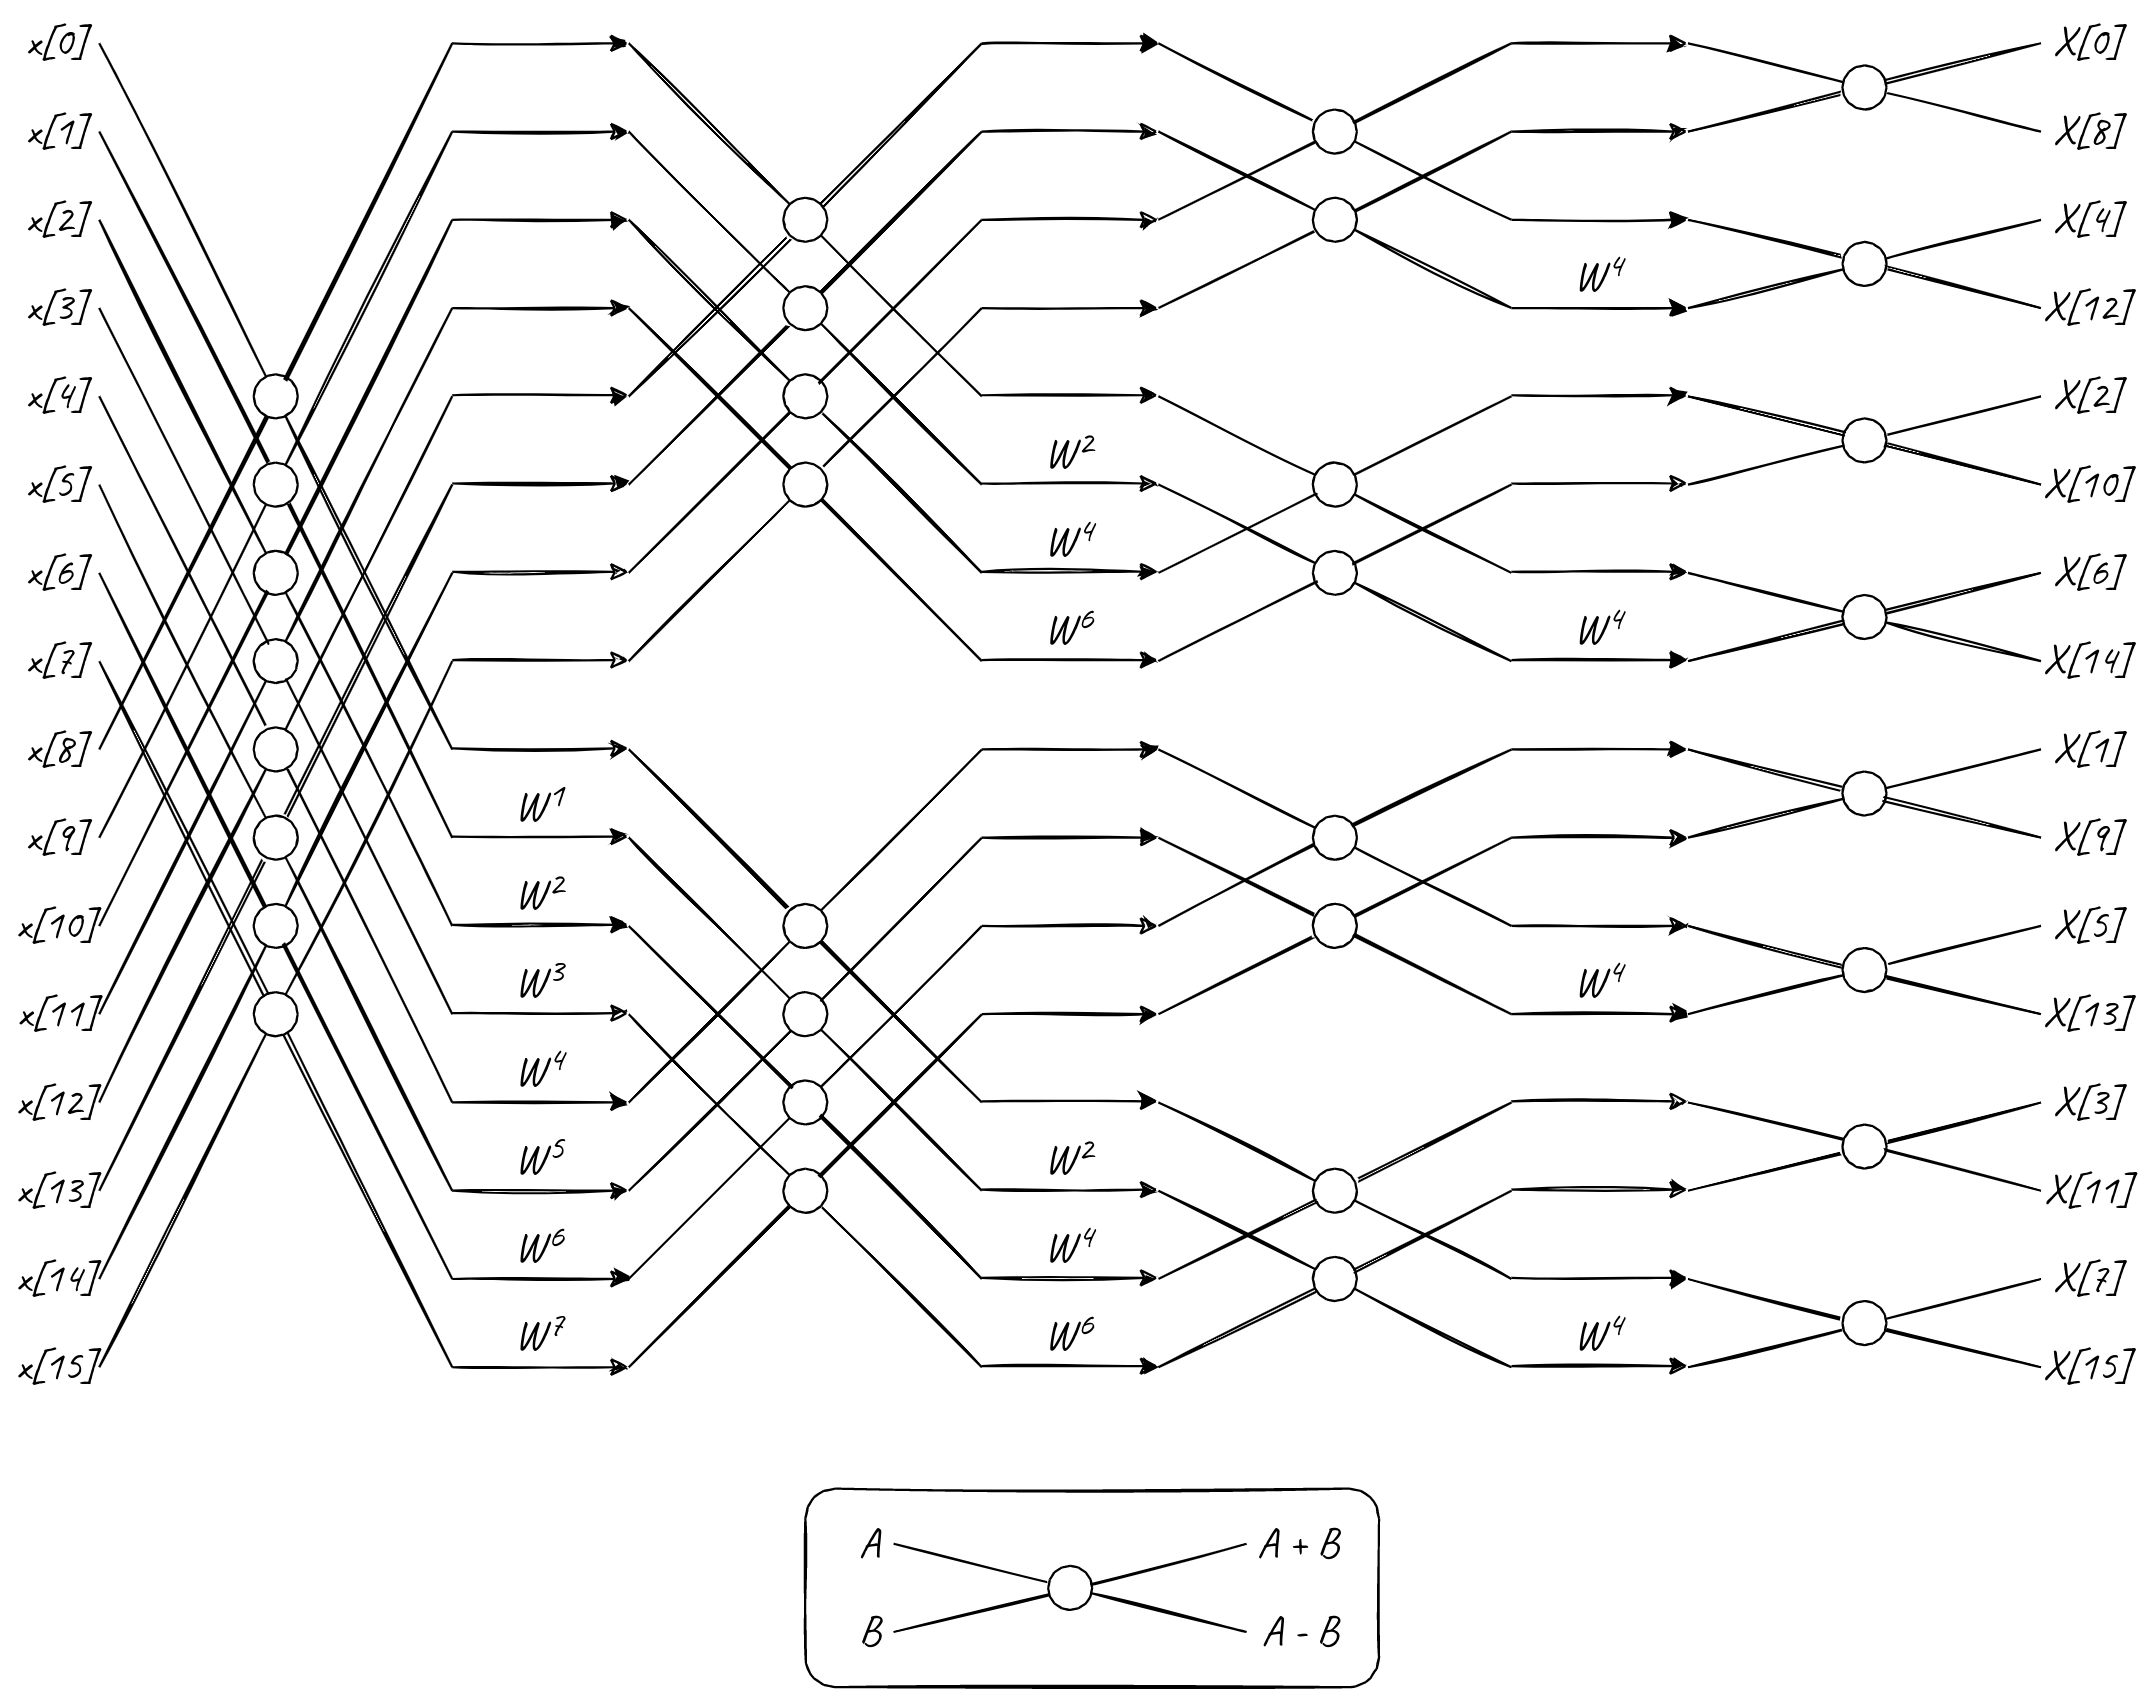
\includegraphics[width=1.\columnwidth]{pics/spring/3/1.png}
	%\caption{.}
	\label{fig:3-1}
\end{figure}

Базовой операцией является двухточечное ДПФ по основанию $2$, состоящее из сложения и вычитания и не содержащее умножений. Все умножения вынесены в поворачивающие множители между итерациями алгоритма. Входные отсчеты должны быть расположены в естественном битовом порядке, а выходные --- в инверсном битовом порядке.

\newpage
\section{}
Изобразить граф алгоритма БПФ с прореживанием \textbf{по времени} для $N=16$. 
Объяснить, в чем заключается базовая операция данного алгоритма.
\begin{figure}[!h]
	\centering
	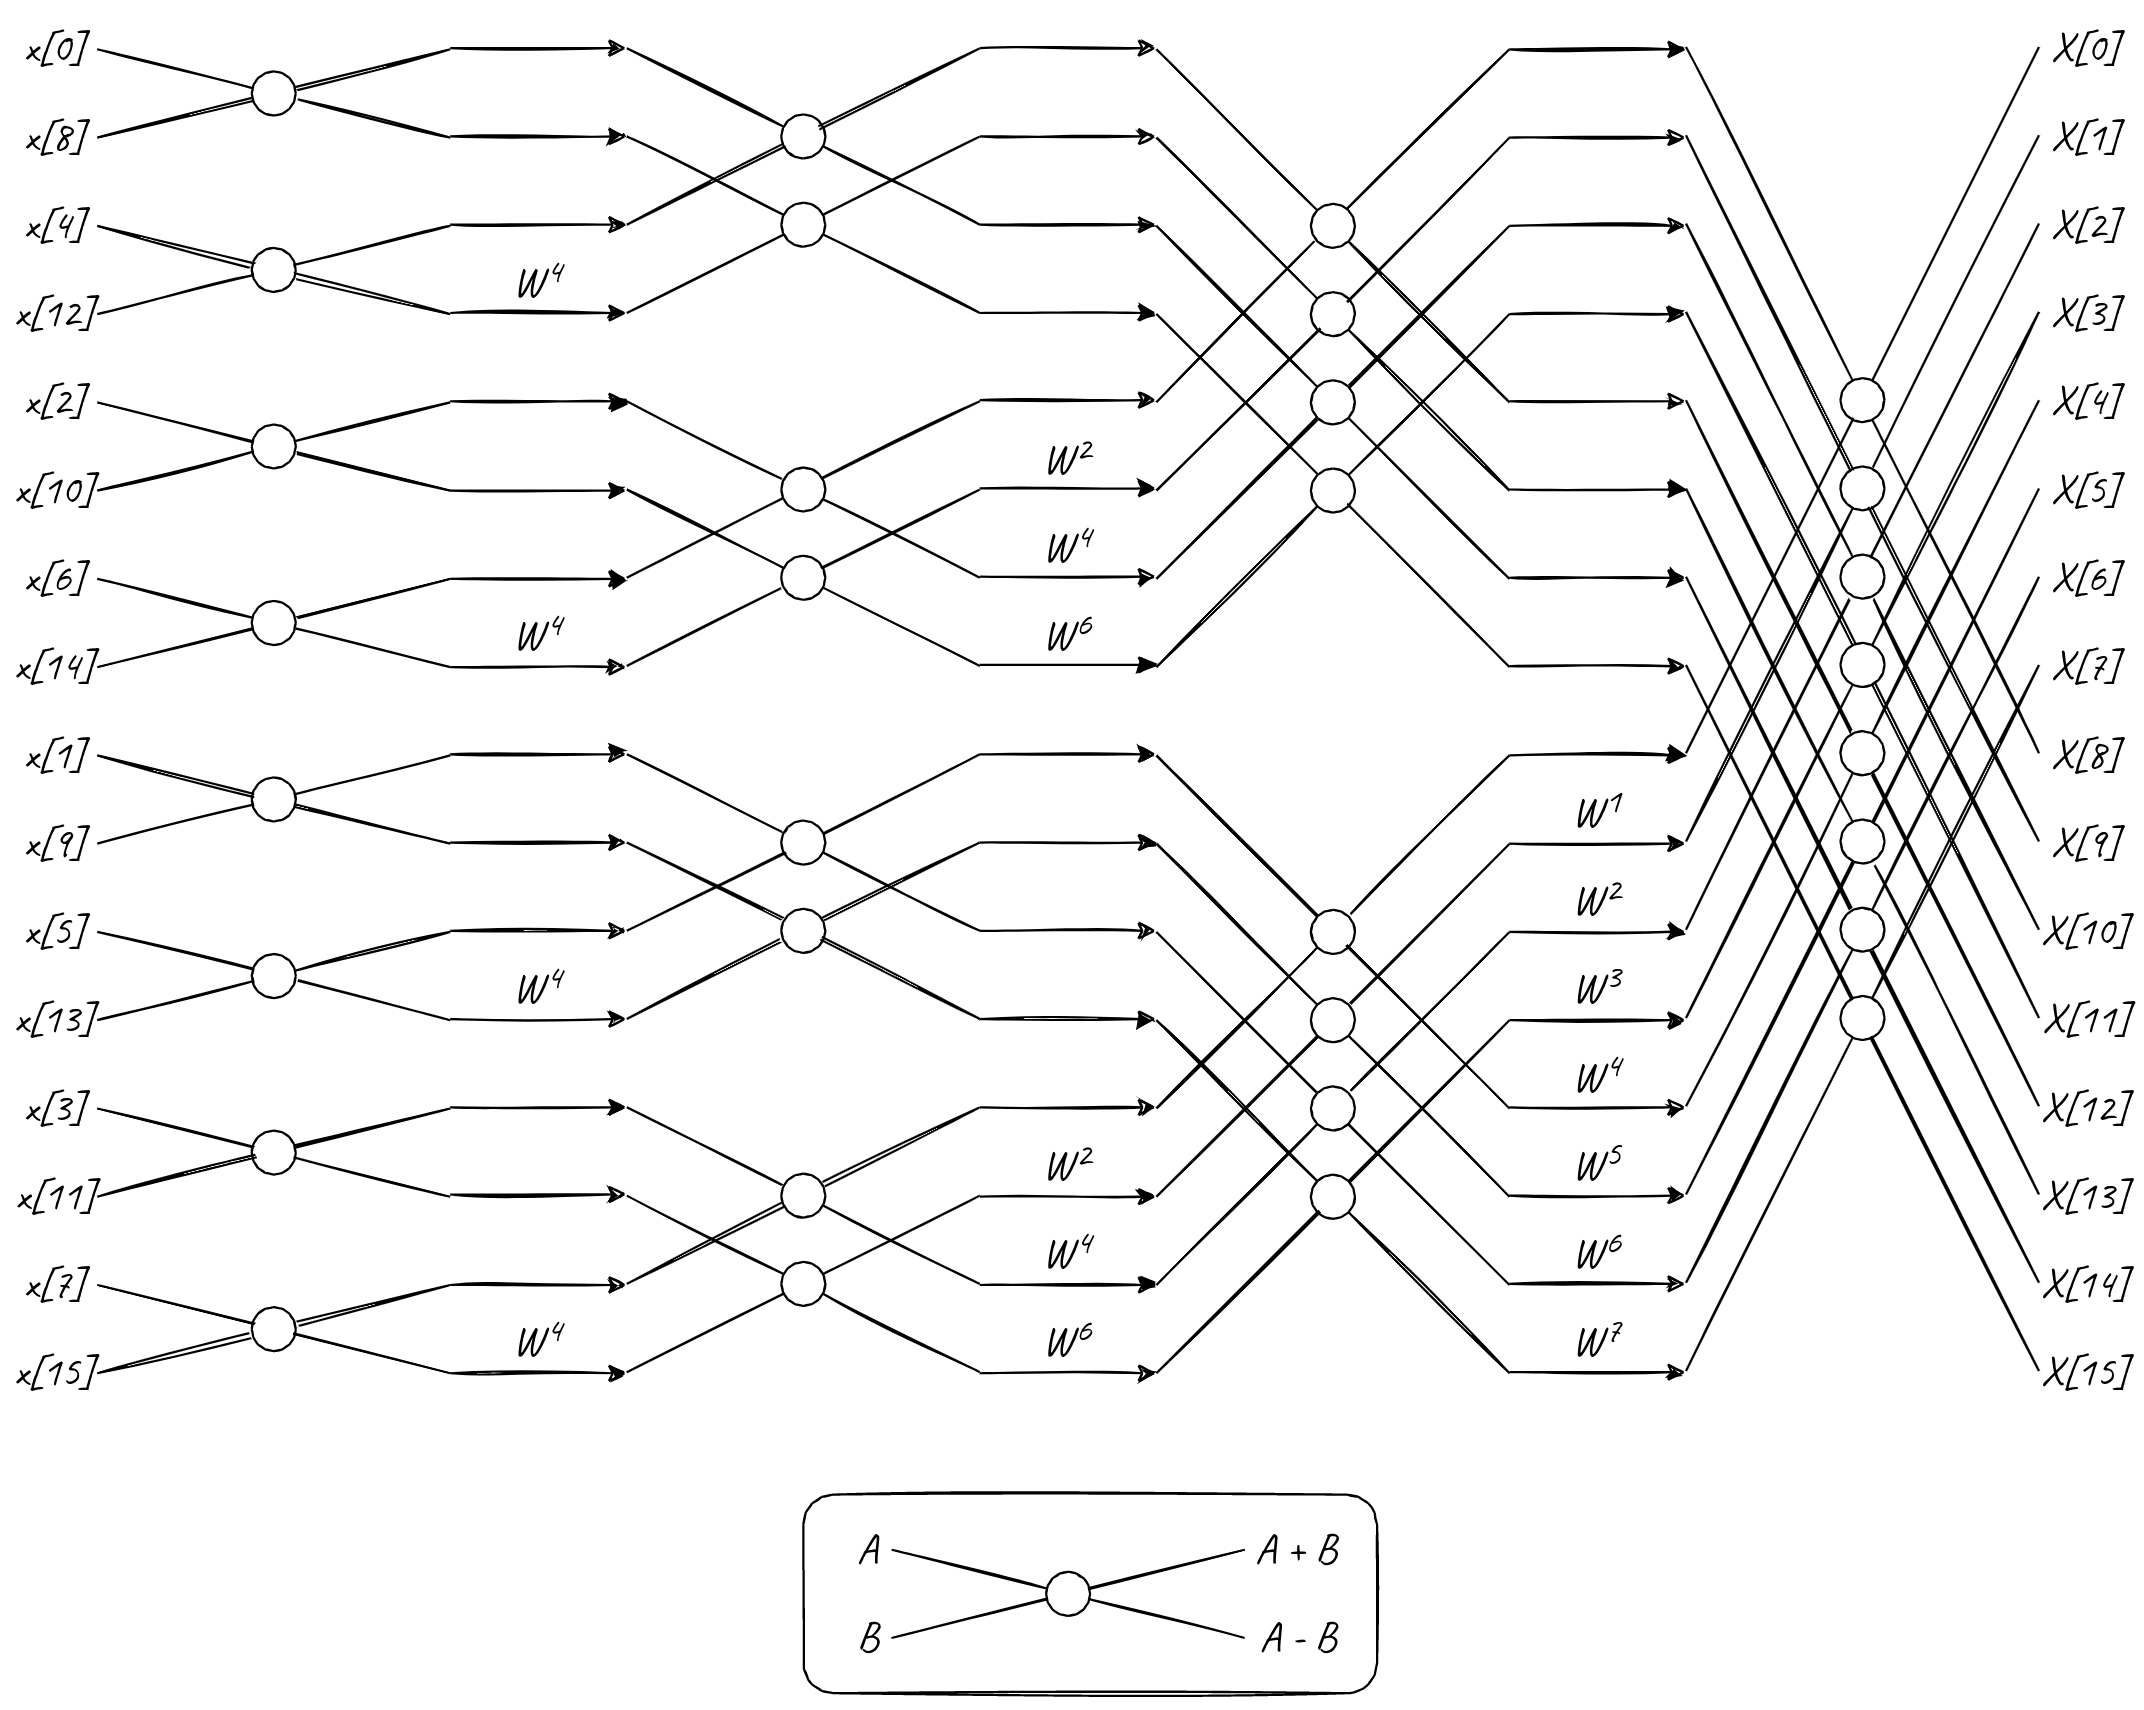
\includegraphics[width=1.\columnwidth]{pics/spring/3/2.png}
	%\caption{.}
	\label{fig:3-2}
\end{figure}

Базовой операцией является двухточечное ДПФ по основанию $2$, состоящее из сложения и вычитания и не содержащее умножений. Все умножения вынесены в поворачивающие множители между итерациями алгоритма. Входные отсчеты должны быть расположены в инверсном битовом порядке, а выходные --- в естественном битовом порядке.



\newpage
\section{}
Записать матрицу, задающую ДПФ преобразование над последовательностью (вектором) длины $4$. Указать матрицу, задающую обратное преобразование. 
В ответе значения всех элементов матрицы должны быть представлены как комплексные числа.

\begin{equation*}
[W_4] =
\begin{bmatrix}
W^0_4 & W^0_4 & W^0_4 & W^0_4\\
W^0_4 & W^1_4 & W^2_4 & W^3_4\\
W^0_4 & W^2_4 & W^4_4 & W^6_4\\
W^0_4 & W^3_4 & W^6_4 & W^9_4
\end{bmatrix} =
\begin{bmatrix}
W^0_4 & W^0_4 & W^0_4 & W^0_4\\
W^0_4 & W^1_4 & W^2_4 & W^3_4\\
W^0_4 & W^2_4 & W^0_4 & W^2_4\\
W^0_4 & W^3_4 & W^2_4 & W^1_4
\end{bmatrix} =
\begin{bmatrix}
+1 & +1 & +1 & +1\\
+1 & -j & -1 & +j\\
+1 & -1 & +1 & -1\\
+1 & +j & -1 & -j
\end{bmatrix}.
\end{equation*}

\begin{equation*}
[W_4]^{-1} = \dfrac{1}{4}[W_4]^{*} = \dfrac{1}{4}
\begin{bmatrix}
+1 & +1 & +1 & +1\\
+1 & +j & -1 & -j\\
+1 & -1 & +1 & -1\\
+1 & -j & -1 & +j
\end{bmatrix}.
\end{equation*}
